\documentclass[a4paper,12pt]{article}
\usepackage[spanish]{babel}
\usepackage[utf8]{inputenc}
\usepackage{booktabs}
\usepackage{dirtytalk}
\usepackage{graphicx}
\usepackage{dirtytalk}
\usepackage[T1]{fontenc}
\usepackage[document]{ragged2e}

\begin{document}

\title{\Large Instituto Politécnico Nacional\\Escuela Superior de Cómputo\\Sistemas Operativos\\ Mapa mental ¿Qu\'e es un sistema operativo? \\Alumno: Meza Zamora Abraham Manuel\\Profesor: Ephra\'in Herrera Salgado}
\date{}
\maketitle

\section{Mapa mental} 
\begin{figure}[h]
\center
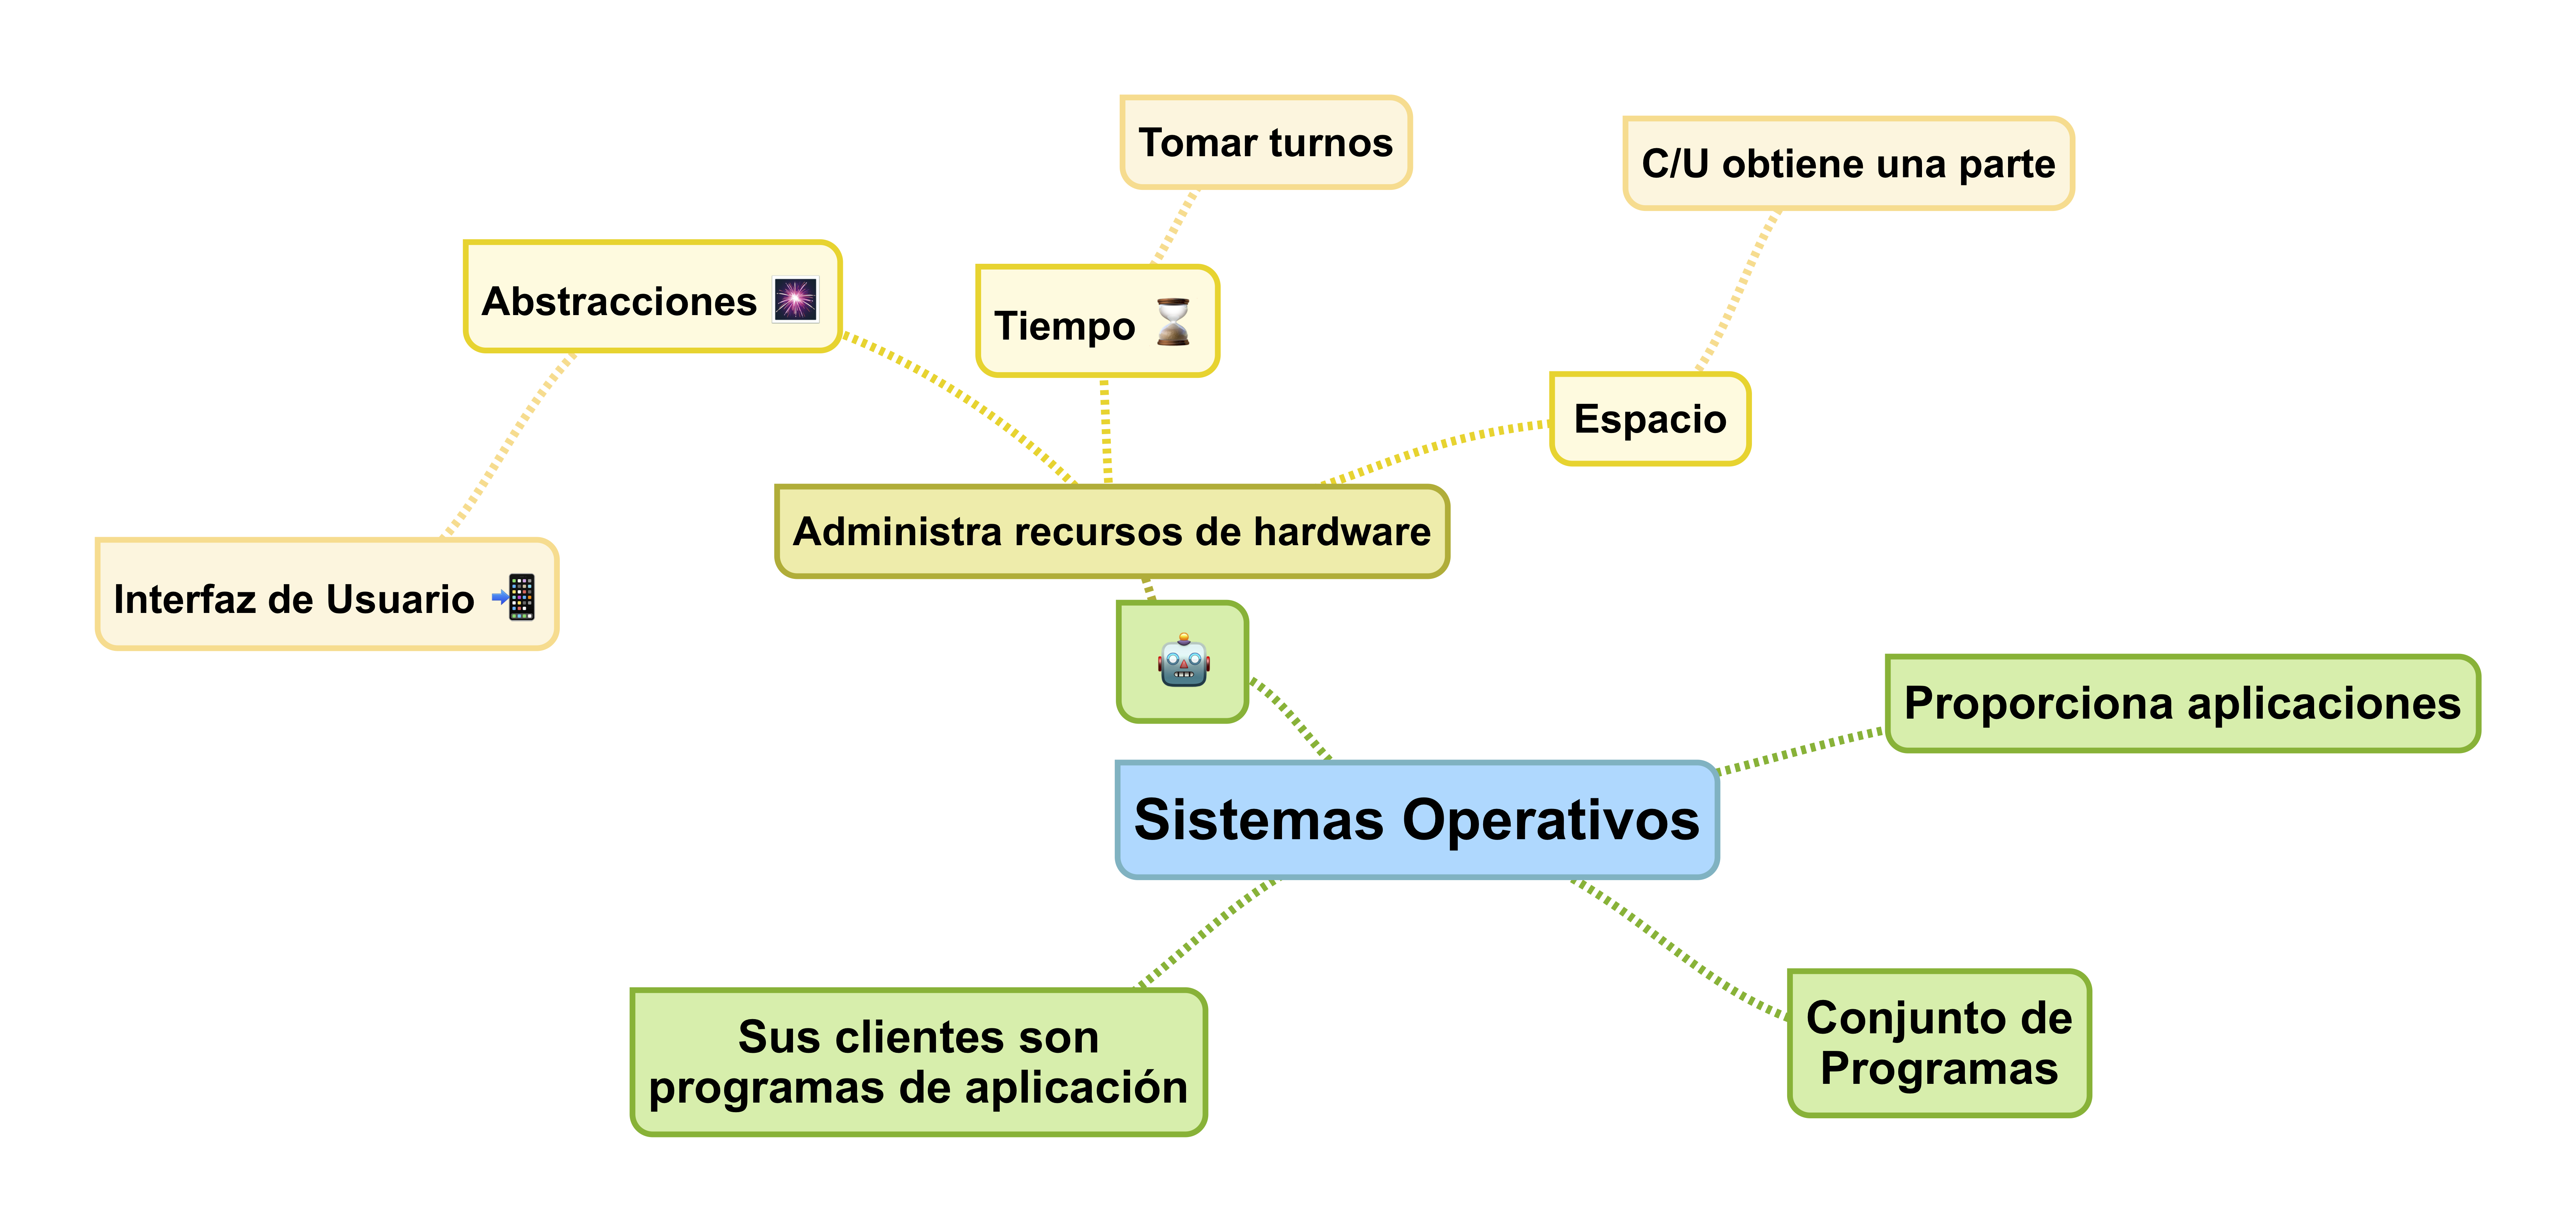
\includegraphics[scale=.75]{SistemasOperativos}
\caption{Mapa mental sistemas operativos.}
\end{figure}
\justify 
Un \textit{sistema operativo} es un conjunto de programas, que proporciona aplicaciones simples al usuario, y se encarga de administrar los recursos y procesos asociados al hardware en tiempo y espacio. Lo anterior se logra mediante abstracciones que permiten al usuario interactuar con la computadora sin entender la parte compleja del hardware. Los clientes del SO son programas de aplicación. 

\end{document}